% !TEX program = lualatex
\documentclass[aspectratio=169,11pt]{beamer}

\usetheme[progressbar=frametitle,numbering=fraction]{metropolis}
\usepackage{luatexja}
\usepackage[haranoaji]{luatexja-preset}
\renewcommand{\kanjifamilydefault}{\gtdefault}
\usepackage{booktabs}
\usepackage{tabularx}
\usepackage{array}
\usepackage{amsmath,amssymb,mathtools}
\usepackage{xurl}
\usepackage{listings}

\newcolumntype{L}{>{\raggedright\arraybackslash}X}
\newcolumntype{R}{>{\raggedleft\arraybackslash}X}

\lstset{basicstyle=\ttfamily\scriptsize, columns=fullflexible, keepspaces=true,
  frame=single, commentstyle=\color{gray}, keywordstyle=\color{blue!60!black}\bfseries,
  morekeywords={set,param,var,binary,minimize,subject,to,sum,in,default}, morecomment=[l]{\#}}

\title{Timefold Facility Location\\AMPL による厳密解との比較}
\subtitle{ロンドン（施設 30・顧客 60）インスタンス}
\date{\today}
\author{}

\begin{document}

\maketitle

\begin{frame}{目次}
  \setbeamertemplate{section in toc}[sections numbered]
  \tableofcontents
\end{frame}

%======================================================================
\section{問題とスコア構造}

\begin{frame}{Timefold Facility Location とは}
  \begin{itemize}
    \item \textbf{出典}: Timefold Quickstarts \texttt{use-cases/facility-location}
    \item \textbf{対象問題}: \alert{単一割当・容量制約付き施設配置問題}（SSCFLP）
    \item 各顧客（需要 15）を施設候補（容量 150）のいずれか\textbf{1 つ}に割り当てる
    \item 1 人でも顧客が割り当てられた施設は「開設」とみなされ，開設費用がかかる
    \item \textbf{目的}: 開設費用と顧客--施設間の距離のバランスをとる
  \end{itemize}
  \vspace{0.5em}
  \begin{block}{インスタンス（ロンドン）}
    施設候補 30（開設費用 33{,}084〜72{,}138，容量 150），顧客 60（需要 15，総需要 900）\\
    $\Rightarrow$ 1 施設あたり最大 10 顧客，最低 6 施設の開設が必要
  \end{block}
\end{frame}

\begin{frame}{Timefold の制約（\texttt{HardSoftScore}）}
  \small
  \begin{tabularx}{\textwidth}{p{50mm}p{15mm}L}
    \toprule
    制約名 & 重み & 内容 \\
    \midrule
    \texttt{facility capacity} & 1 hard & 施設の割当需要合計が容量を超えた分をペナルティ \\
    \texttt{facility setup cost} & 2 soft & 使用された施設の開設費用 \texttt{setupCost} \\
    \texttt{distance from facility} & 6 soft & 顧客と割当施設の距離 [m]（既定 5 を 6 に上書き） \\
    \bottomrule
  \end{tabularx}
  \vspace{0.8em}
  \begin{block}{距離の定義（\texttt{Location.getDistanceTo}）}
    緯度経度を平面座標とみなしたユークリッド距離に $111{,}000$ m/度 を掛けて切り上げ
    \[
      d_{ij} = \left\lceil 111000 \sqrt{(\phi_i-\phi_j)^2 + (\lambda_i-\lambda_j)^2}\,\right\rceil
    \]
  \end{block}
\end{frame}

%======================================================================
\section{数理定式化と AMPL モデル}

\begin{frame}{0-1 整数計画としての定式化}
  \begin{columns}[T]
    \begin{column}{0.48\textwidth}
      \small
      \textbf{集合・パラメータ}
      \begin{itemize}
        \item $J$: 施設候補，$I$: 顧客
        \item $f_j$: 開設費用，$u_j$: 容量
        \item $q_i$: 需要，$d_{ij}$: 距離 [m]
        \item $w_f = 2,\ w_d = 6$: 制約重み
      \end{itemize}
      \textbf{変数}
      \begin{itemize}
        \item $y_j \in \{0,1\}$: 施設 $j$ を開設
        \item $x_{ij} \in \{0,1\}$: 顧客 $i$ を施設 $j$ に割当
      \end{itemize}
    \end{column}
    \begin{column}{0.52\textwidth}
      \small
      \begin{align*}
        \min\ & w_f \sum_{j} f_j y_j + w_d \sum_{i,j} d_{ij} x_{ij} \\
        \text{s.t. }
        & \textstyle\sum_{j} x_{ij} = 1 && \forall i \\
        & \textstyle\sum_{i} q_i x_{ij} \le u_j y_j && \forall j \\
        & x_{ij} \le y_j && \forall i,j
      \end{align*}
      \begin{itemize}
        \item 目的関数 $=$ Timefold の $-$soft スコア
        \item hard 制約（容量）は\alert{制約として厳守}
        \item 最終式は冗長だが LP 緩和を強化
      \end{itemize}
    \end{column}
  \end{columns}
\end{frame}

\begin{frame}[fragile]{AMPL モデル \texttt{cflp.mod}}
\begin{lstlisting}
set FAC;  set CUS;
param setup {FAC} >= 0;  param cap {FAC} >= 0;
param dem {CUS} >= 0;    param dist {CUS, FAC} >= 0;
param w_setup default 2; param w_dist default 6;

var y {FAC} binary;
var x {CUS, FAC} binary;

minimize SoftCost:
    w_setup * sum {j in FAC} setup[j] * y[j]
  + w_dist  * sum {i in CUS, j in FAC} dist[i,j] * x[i,j];

subject to Assign {i in CUS}:   sum {j in FAC} x[i,j] = 1;
subject to Capacity {j in FAC}: sum {i in CUS} dem[i] * x[i,j] <= cap[j] * y[j];
subject to Link {i in CUS, j in FAC}: x[i,j] <= y[j];   # 強い定式化
\end{lstlisting}
  \small 変数 $30 + 1{,}800 = 1{,}830$ 個，制約 $60 + 30 + 1{,}800 = 1{,}890$ 本
\end{frame}

\begin{frame}[fragile]{amplpy による求解（\texttt{solve\_cflp.py}）}
\begin{lstlisting}[language=Python, morekeywords={def,return,for,in,import,from}]
P = json.load(open("london.json"))["problem"]          # Timefold UI の保存データ
F = {f["id"]: f for f in P["facilities"]}
C = {c["id"]: c for c in P["consumers"]}
D = {(i, j): distance(C[i]["location"], F[j]["location"]) for i in C for j in F}

ampl = AMPL(); ampl.read("cflp.mod")
ampl.set["FAC"] = list(F);  ampl.set["CUS"] = list(C)
ampl.param["setup"] = {j: F[j]["setupCost"] for j in F}
ampl.param["cap"]   = {j: F[j]["capacity"]  for j in F}
ampl.param["dem"]   = {i: C[i]["demand"]    for i in C}
ampl.param["dist"]  = D
ampl.option["solver"] = "gurobi"          # または "highs"
ampl.solve()
\end{lstlisting}
  \small
  JSON に含まれる Timefold の割当（\texttt{consumer.facility}）からスコアを再計算し，
  保存値 \texttt{0hard/-1510342soft} と\alert{完全一致}することを確認した上で比較
\end{frame}

%======================================================================
\section{計算結果}

\begin{frame}{Timefold 解と AMPL 最適解の比較}
  \small
  \begin{tabularx}{\textwidth}{L R R R}
    \toprule
    & Timefold & AMPL（最適） & 差（AMPL$-$TF） \\
    \midrule
    hard スコア & 0 & 0 & 0 \\
    soft スコア & $-1{,}510{,}342$ & $-1{,}467{,}636$ & $+42{,}706$ \\
    開設施設数 & 7 & 7 & 0 \\
    開設費用合計 & 313,178 & 311,028 & $-2{,}150$ \\
    \quad $\times 2$（soft 寄与） & 626,356 & 622,056 & $-4{,}300$ \\
    距離合計 [m] & 147,331 & 140,930 & $-6{,}401$ \\
    \quad $\times 6$（soft 寄与） & 883,986 & 845,580 & $-38{,}406$ \\
    \bottomrule
  \end{tabularx}
  \vspace{0.8em}
  \begin{itemize}
    \item Timefold 解は最適値より \alert{2.91\%} 悪い（実行可能だが最適ではない）
    \item 改善の約 9 割は\textbf{距離項}から（総距離 4.3\% 短縮）
    \item 割当が変わった顧客: 60 人中 18 人
  \end{itemize}
\end{frame}

\begin{frame}{開設施設と割当負荷}
  \small
  \begin{columns}[T]
    \begin{column}{0.48\textwidth}
      \centering\textbf{Timefold}\\[0.3em]
      \begin{tabular}{rrr}
        \toprule
        施設 & 開設費用 & 割当需要 \\
        \midrule
        10 & 42,682 & 90 \\
        11 & 46,001 & 135 \\
        \alert{13} & 46,095 & 150 \\
        15 & 43,421 & 135 \\
        22 & 33,084 & 135 \\
        25 & 54,049 & 150 \\
        \alert{26} & 47,846 & 105 \\
        \bottomrule
      \end{tabular}
    \end{column}
    \begin{column}{0.48\textwidth}
      \centering\textbf{AMPL 最適解}\\[0.3em]
      \begin{tabular}{rrr}
        \toprule
        施設 & 開設費用 & 割当需要 \\
        \midrule
        10 & 42,682 & 105 \\
        11 & 46,001 & 135 \\
        15 & 43,421 & 150 \\
        \alert{19} & 48,631 & 120 \\
        22 & 33,084 & 150 \\
        \alert{24} & 43,160 & 90 \\
        25 & 54,049 & 150 \\
        \bottomrule
      \end{tabular}
    \end{column}
  \end{columns}
  \vspace{0.8em}
  \centering
  5 施設は共通．北部の \{13, 26\} を \{19, 24\} に入れ替えることで開設費用・距離の両方が減少
\end{frame}

\begin{frame}{割当の可視化}
  \centering\vspace*{-0.5em}
  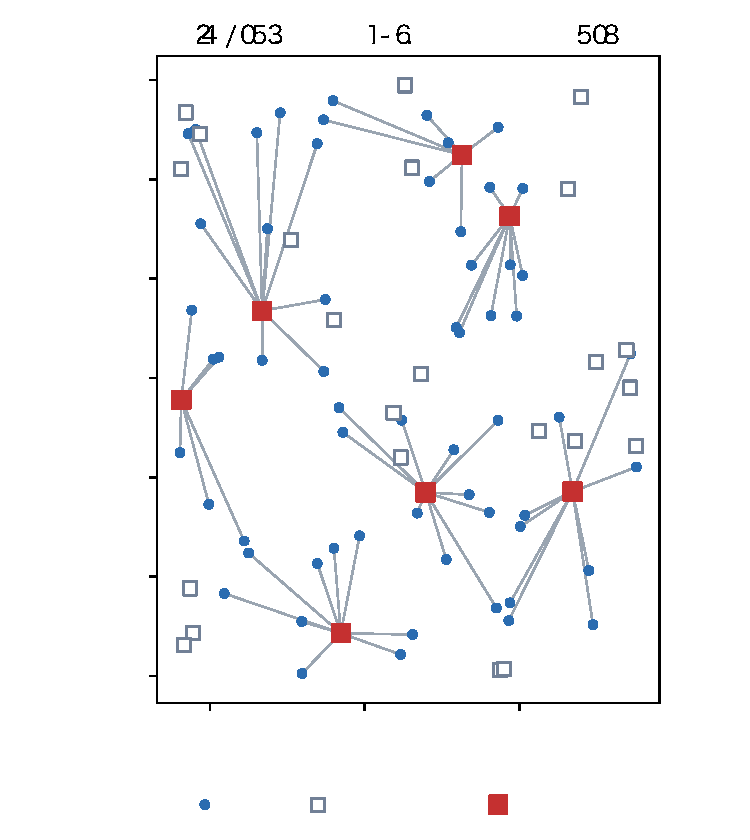
\includegraphics[height=0.86\textheight]{results/timefold_map.pdf}\hfill
  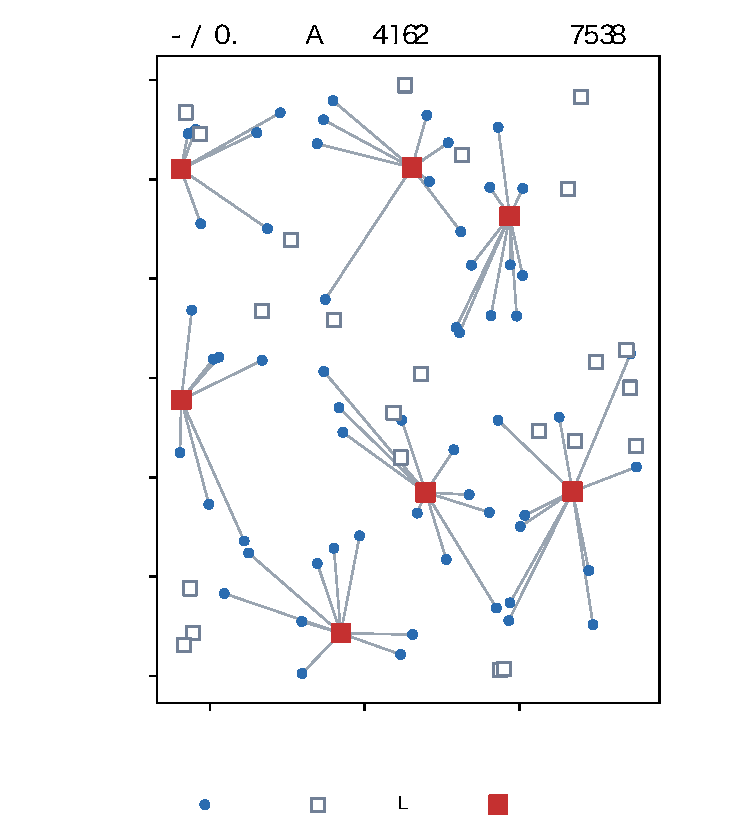
\includegraphics[height=0.86\textheight]{results/ampl_map.pdf}
\end{frame}

\begin{frame}{ソルバー性能と定式化の強さ}
  \small
  \begin{tabularx}{\textwidth}{l l R R R}
    \toprule
    ソルバー & 定式化 & LP 緩和値 & LP ギャップ & 求解時間 [s] \\
    \midrule
    Gurobi & 強（$x_{ij}\le y_j$ あり） & 1,460,251.8 & 0.50\% & 0.22 \\
    Gurobi & 弱（容量制約のみ） & 1,145,689.0 & 21.94\% & 0.32 \\
    HiGHS 1.11 & 強 & 1,460,251.8 & 0.50\% & 1.42 \\
    HiGHS 1.11 & 弱 & 1,145,689.0 & 21.94\% & 1.26 \\
    \bottomrule
  \end{tabularx}
  \vspace{0.8em}
  \begin{itemize}
    \item 全ケースで同じ最適値 1,467,636 に到達し，最適性が証明された
    \item 強い定式化は LP 緩和がほぼ整数解に近く，HiGHS は分枝 1 ノードで終了
    \item 求解時間は AMPL 呼び出しを含む実時間（ローカル環境，1 回計測）
  \end{itemize}
\end{frame}

%======================================================================
\section{まとめ}

\begin{frame}{まとめ}
  \begin{itemize}
    \item Timefold facility-location のスコアを 0-1 整数計画（SSCFLP）として\textbf{厳密に再現}
    \item 施設 30・顧客 60 の規模では AMPL + Gurobi / HiGHS が\alert{1 秒前後で最適解}を算出
    \item Timefold 解は実行可能（0hard）だが soft スコアで最適値から 2.91\% の差
    \begin{itemize}
      \item 開設施設 2 か所の入れ替えと 18 顧客の再割当で改善
    \end{itemize}
    \item 冗長制約 $x_{ij} \le y_j$ により LP ギャップは 21.9\% $\to$ 0.5\% に縮小
    \item 大規模インスタンスでは Timefold（局所探索）と MIP（厳密解・下界）を
          \textbf{併用}し，下界で Timefold 解の品質を評価するのが有効
  \end{itemize}
  \vspace{0.5em}
  \begin{block}{ファイル}
    \footnotesize
    \texttt{facility/cflp.mod}，\texttt{facility/solve\_cflp.py}，\texttt{facility/london.json}，\texttt{facility/results/}
  \end{block}
\end{frame}

\end{document}
